\chapter{Divisibilidade}
\label{chap:div}

Nesse capítulo apresentamos os principais conceitos relacionados
à divisão.

\section{Divisão Euclidiana}

Sejam $a, b \in \ZZ$ tais que $b \neq 0$.
Pela divisão euclidiana sabemos que é possível dividir
$a$ por $b$ e, como resultado, obtemos $q, r$ inteiros tais que
$0\leq r < b$ tais que
$$
  a = bq + r
$$
Além disso os inteiros $q$ e $r$ são únicos com essa
propriedade. Vamos relembrar a demonstração desse fato.
\begin{proof}
  Considere o conjunto $R = \{a-bk\mid k \in \ZZ\}$. Note que,
  como $b \neq 0$, o conjunto $R$ é infinito. Na verdade, podemos
  considerar o conjunto $R$ como uma progressão aritmética
  \emph{nas duas direções} com termo inicial $a$ e razão $b$.
  Dessa forma, temos que $S\cap \ZZ_{\geq 0} \neq \emptyset$.
  Pelo princípio da boa ordenação existe portanto
  um elemento minimal em $R$, digamos $r_0 = a-bk_0$ para
  algum $k_0 \in \ZZ$. Temos então que 
  $$
    a = r_0 + bk_0
  $$
  Por definição temos que $r_0 \geq 0$. Vale também
  que $r_0 <|b|$, caso contrário $0<r_0 - |b| = a+b(k_0 \pm 1)$ 
  seria um elemento de $S\cap \ZZ_{\geq 0}$
  menor que $r_0$, contradizendo
  a minimalidade de $r_0$.
  Portanto $r = r_0$ e $q = k_0$ satisfazem a hipótese 
  desejada. A unicidade do par $q$ e $r$ fica como
  exercício para o leitor.
\end{proof}


Obviamente o \Sage já possui um comando que calcula,
dados  inteiros $a$ e $b\neq 0$, o quociente $q$
e o resto $r$ da divisão de $a$ por $b$. Contudo, vamos
aproveitar esse simples problema para nos
familiarizar com o \sage. Usaremos os conceitos
básicos de listas.

Como vimos, o
conjunto $R$ na demonstração é infinito, então não podemos
representá-lo no \Sage (pelo menos não como uma lista). Fixemos $a = 10$
e $b = 3$ e listemos
os elementos de $R$ com $k$ variando de $-5$ a $5$,
para isso usaremos a construção por compreensão de listas,
apresentada na Introdução.

\begin{sageinput}
a = 10
b = 3
[a-k*b for k in srange(-5,6)]
\end{sageinput}
\begin{sageoutput}
[25, 22, 19, 16, 13, 10, 7, 4, 1, -2, -5]
\end{sageoutput}

Note que o menor elemento não negativo na lista
é o $1$, que é, de fato, o resto da divisão de $a = 10$ por
$b = 3$, já que $10 = 3\times 3 + 1$ e $0\leq r = 1 < 3$.
No entanto, ainda que seja possível capturar através
do \Sage o menor elemento positivo de uma lista, essa
tecnica pode não funcionar. Tente criar o subconjunto
análogo de $S$ para $a = 1932$ e $b = 7$.

Podemos resolver esse problema usando o \emph{laço
de repetição} \ils{while}. Ao invés
de criar um subconjunto de $R$ e procurarmos ali
o menor não negativo, começamos do $a$; isto é, $k = 0$,
e caminhamos na direção certa para encontrar
o resto. Note que a "direção  certa"\ depende
dos sinais de $a$ e $b$. Por exemplo, se
tomarmos $a = 10$ e $b = -3$:

\begin{sageinput}
a = 10                                                                                             
b = -3                                                                                             
[a-k*b for k in srange(-5,6)]                                                                      
\end{sageinput}
\begin{sageoutput}
[-5, -2, 1, 4, 7, 10, 13, 16, 19, 22, 25]
\end{sageoutput}
\noindent A lista está no sentido oposto à anterior! Assim, a partir
do $10$ devemos caminhar para trás tomando 
$k =-1,-2, \dots$, para encontrar o menor não negativo.
Tome $a = 39$ e $b = 4$. A célula a seguir
toma $k = 0, 1, 2, \dots$ testando o valor de $a-kb$. 
Se chegarmos à um valor negativo para determinado
$k$ então o menor não negativo foi obtido no passo anterior.
\begin{sageinput}
a = 39
b = 4
k = 0
while a-(k+1)*b >= 0:
  k += 1
print("Quociente:", k)
print("Resto:", a-k*b)
\end{sageinput}
\begin{sageoutput}
Quociente: 9
Resto:  3
\end{sageoutput}


% coincidindo com o sage.
% \begin{sageinput}
% def div_euc(a,b):
%   k = 0
%   if a == 0:
%     return (0,0)
%   if a > 0 and b > 0:
%     while a-k*b >= 0:
%       k += 1
%     return (k-1, a-(k-1)*b)
%   elif a < 0 and b > 0:
%     while a-k*b <= 0:
%       k += 1
%     return (k, a-k*b)
%   elif a < 0 and b < 0:
%     while a-k*b <= 0:
%       k += 1
%     return (k-1, a-(k-1)*b)
%   else:
%   #a > 0 e b < 0
%     while a-k*b >= 0:
%       k -= 1
%     return (k, a-(k)*b)
% \end{sageinput}
% \begin{sageoutput}
%   output
% \end{sageoutput}

Teste esse código com outros valores para $a$ e $b$. Mas
cuidado! Se você trocar o sinal de $b$ o seu algoritmo não
vai terminar nunca (por que?). Vejamos com calma o que está
acontecendo. Nas primeiras três linhas apenas atribuímos
os valores de $a, b$ e o valor inicial de $k$. Na linha
$4$ criamos um laço de repetição que testa se o número 
$a-(k+1)b$ é não negativo. Caso seja, passamos para o
próximo valor de $k$ na linha seguinte
e voltamos para a linha com o \ils{while}, testando novamente. Caso o valor
obtido seja negativo, isso implica que o menor natural
não negativo é o $a-kb$, que é o resto, e o quociente
é o $k$. As demais linhas apenas exibem o resultado.
Nos exercícios você deverá criar um algoritmo
parecido para os demais possibilidades de sinal de $a$ e $b$.

Obviamente o \Sage já possui uma ferramenta para 
o cálculo do quociente e do resto, o método
\ils{.quo\_rem} da classe \ils{Integer}.
\index[sage]{\ils{.quo\_rem}}
\begin{sageinput}
a = 39
b = 4
a.quo_rem(b)
\end{sageinput}
\begin{sageoutput}
(9, 3)
\end{sageoutput}

O retorno é uma tupla onde o primeiro elemento
é o quociente e o segundo é o resto... Bem, quase
isso: esse método tem um comportamento que 
requer certo cuidado. Pela nossa definição, o resto
\textbf{deve ser não negativo}. No entanto, o 
\ils{.quo\_rem} retorna um resto negativo
quando $b<0$. 
\begin{sageinput}
39.quo_rem(-4)                                                                                     
\end{sageinput}
\begin{sageoutput}
(-10, -1)
\end{sageoutput}

De fato, $39 = (-10)(-4)-1$ mas isso não é 
a nossa divisão euclidiana de $39$ por $-4$, e
sim $39 = (-9)(-4)+3$ pois $0\leq r = 3 < |-4| = 4$.
Uma forma mais direta de se encontrar
o resto é usar o operador \ils{\%}.

\begin{sageinput}
39 % 4
\end{sageinput}
\begin{sageoutput}
3
\end{sageoutput}
No entanto ainda temos um resto negativo quando $b<0$. 
Uma maneira de se obter o resto no intervalo esperado
é usar o método \ils{.mod}. \index[sage]{\ils{.mod}}
\begin{sageinput}
mod(39,-4)
\end{sageinput}
\begin{sageoutput}
3
\end{sageoutput}
Discutiremos esse método nos próximos capítulos, mas 
destacamos que o resultado retornado pelo \ils{.mod}
não é um inteiro (você pode descobrir o tipo 
de um objeto com a função \ils{parent}, tente!).
\index[sage]{\ils{parent}}

Quando o resto da divisão euclidiana de $a$ por $b$
é zero dizemos que \emph{$b$ divide $a$} e denotamos
essa relação por $b\mid a$. O \Sage sabe
nos dizer quando isso acontece:
\begin{sageinput}
2.divides(37); 5.divides(25)
\end{sageinput}
\begin{sageoutput}
False
True
\end{sageoutput}

Se $b$ divide $a$ dizemos que $b$ é um \emph{divisor}
ou \emph{fator} de $a$, ou que $a$ é um múltiplo de $b$.
O \Sage consegue encontrar todos os divisores 
de um número dado com a função \ils{divisors}.
\index[sage]{\ils{divisors}}

\begin{sageinput}
divisors(12) ; divisors(7)
\end{sageinput}
\begin{sageoutput}
[1, 2, 3, 4, 6, 12]
[1, 7]
\end{sageoutput}

Note que a lista contém apenas os divisores positivos,
mas, pela nossa definição, segue que se $b\mid a$
então $-b\mid a$, de forma que os negativos também
são considerados divisores.

\section{Primos}


Esse é um bom momento para relembrar a definição
de número primo. Um natural $p>1$ é dito 
\emph{primo}\index{Número!primo} se seus únicos divisores positivos são $1$ ou $p$.
Você poderia testar se um número $n$ é primo verificando
se sua lista de divisores é \ils{[1,p]}, mas
o método \ils{.is\_prime} já faz isso:
\index[sage]{\ils{is\_prime}}
\begin{sageinput}
12.is_prime() ; 19.is_prime()
\end{sageinput}
\begin{sageoutput}
False
True
\end{sageoutput}

Números primos são extremamente importantes na teoria dos
números. Apresentamos algumas ferramentas
do \Sage envolvendo primos. Além de verificar se um dado natural 
é primo o \Sage consegue gerar e listar os primos. A função
\ils{primes\_first\_n(n)} retorna os $n$ primeiros primos,
a função \ils{primes(a,b)} retorna os primos entre $a$ e $b-1$
e \ils{random\_prime(n)} retorna um primo aleatório menor
ou igual a $n$. Vejamos alguns exemplos
\index[sage]{\ils{primes\_first\_n}}
\index[sage]{\ils{primes}}
\index[sage]{\ils{random\_prime}}

\begin{sageinput}
print("Os 10 primeiros primos sao", primes_first_n(10))
print("Os primos entre 50 e 80 sao", list(primes(50, 81)))
print("Um primo menor que 10^10:", random_prime(10^10))
\end{sageinput}
\begin{sageoutput}
Os 10 primeiros primos sao [2, 3, 5, 7, 11, 13, 17, 19, 23, 29]
Os primos entre 50 e 80 sao [53, 59, 61, 67, 71, 73, 79]
Um primo menor que 10^10: 3943466743
\end{sageoutput}

O comando \ils{primes(a,b)} na verdade não retorna uma lista, 
e sim um objeto iterável, não importa muito agora o que isso
significa, mas você deve saber que podemos transformá-lo
em uma lista, 
como vimos no exemplo. A função \ils{random\_prime} será
bastante útil nas nossas investigações, com ela podemos
também passar um limite inferior para o primo desejado,
usando o parâmetro \ils{lbound}, de forma que
\ils{random\_prime(a,lbound=b)} irá retornar um 
primo entre $a$ e $b$.

\begin{sageinput}
random_prime(10^20, lbound=10^19)
\end{sageinput}
\begin{sageoutput}
27132302867607456901
\end{sageoutput}

Note que esse comando é equivalente a escolher
um elemento aleatório da lista dos primos entre
$10^{19}$ e $10^{20}$. Isso pode ser feito com
a função \ils{choice}, que escolhe \index[sage]{\ils{choice}}
um elemento aleatório de uma lista,
nosso comando então seria
da forma {\ils{choice(list(primes(a,b+1)))}}. 
Contudo esse método é bem mais lento pois 
gera todos os primos entre $a$ e $b$ para depois escolher
um deles aleatoriamente.
Obviamente, métodos envolvendo uma escolha aleatória irão
retornar resultados possivelmente diferentes cada vez
que forem executados. A possibilidade de gerar
primos, sobretudo primos com muitos dígitos, é essencial
para a criptografia, como discutiremos na seção \ref{sec:cripto}

Os métodos envolvendo primos, como o \ils{.is\_prime()},
e diversos outros métodos de aritmética, podem se tornar 
mais eficientes se permitimos que eles utilizem 
algoritmos probabilísticos. Isso significa que existe uma
probabilidade muito muito muito baixa de tais métodos
retornarem resultados errados, por exemplo, um número composto
para  \ils{.random\_prime()}.
Existe uma forma de avisar ao \Sage
se você prefere ou não utilizar algoritmos probabilísticos ou
resultados não provados em seus cálculos através da
função \ils{proof.arithmetic()}, veja
\cite[Global proof preferences]{sagedoc}. Discutiremos
brevemente a ideia de pseudoprimo e do funcionamento 
de algoritmos probabilísticos no capítulo \ref{chap:primos}.


\section{MDC}
\label{sec:mdc}
Um dos conceitos mais importantes da aritmética básica
é o de \emph{máximo divisor comum}\index{MDC}: Dados dois inteiros
$a$ e $b$ não ambos nulos, o máximo divisor comum
entre $a$ e $b$, denotado por $\mdc(a,b), \gcd(a,b)$
ou simplesmente $(a,b)$, é o maior inteiro
possível dividindo ambos $a$ e $b$, é portanto 
o maior elemento possível da interseção entre
o conjunto dos divisores de $a$ e de $b$.
Como esses conjuntos são finitos e $1$ pertence
a ambos os conjuntos, o $\mdc$ é sempre um
inteiro positivo. Se $\mdc(a,b) = 1$
dizemos que $a$ e $b$ são \emph{coprimos, relativamente
primos ou primos entre si}.

Podemos encontrar o $\mdc$ entre $a$
e $b$ no \Sage encontrando o maior elemento presente
em ambas as listas \ils{divisors(a)} e \ils{divisors(b)}. 
Vejamos uma forma de fazer isso:
\begin{sageinput}
a = 324
b = 212
max([d for d in divisors(a) if d in divisors(b)])
\end{sageinput}
\begin{sageoutput}
4
\end{sageoutput}
A compreensão de listas\index{Compreensão de listas}
cria uma lista nova com os elementos
de \ils{divisors(a)} que estão também em \ils{divisors(b)},
ou seja, a interseção de tais listas, em seguida,
usando a função \ils{max}, encontramos
o maior elemento dessa lista, obtendo portanto o $\mdc(a,b)$.
Como não poderia deixar de ser, o $\Sage$ já possui uma
função que calcula o mdc, o \ils{gcd}:\index[sage]{\ils{mdc}}
\begin{sageinput}
gcd(324,212)
\end{sageinput}
\begin{sageoutput}
4
\end{sageoutput}

Há uma questão que evitamos até agora mas esse é um
bom momento para discutir. Será que o que estamos fazendo
é eficiente? Por exemplo, para descobrir o $\mdc$ acima
fizemos a interseção entre os divisores de $a$ e de $b$.
Porém, encontrar a lista dos divisores de um número
é equivalente a encontrar sua fatoração em primos e,
como veremos mais adiante, fatorar um número pode
ser muito lento se o número for muito grande. Como
um teste, tente calcular o  $\mdc(10^{50}+1, 10^{49}-1)$
usando a interseção de listas e usando o comando
\ils{gcd}. Você deverá notar que o comando
nativo $\ils{gcd}$ é muito mais rápido. Isso acontece
pois o \Sage está usando internamente o 
\emph{algoritmo de Euclides} para o cálculo do mdc.
\index{Algoritmo! Euclides, cálculo do $\mdc$}
Antes de apresentar tal algoritmo, um lema.

\begin{lemma}
  \label{lemma:mdc}
  Sejam $a, b \in \ZZ$ não ambos nulos. Então
  $\mdc(a,b) = \mdc(b,a-kb)$ para todo $k \in \ZZ$.
  Em particular, se $r$ é o resto da divisão
  euclidiana de $a$ por $b$, então
  $\mdc(a,b) = \mdc(b,r)$.
\end{lemma}
\begin{proof}
  Exercício.
\end{proof}

Como o resto da divisão de $a$ por $b$ é necessariamente
menor que $|b|$, na prática estamos trocando o cálculo do $\mdc$
desejado pelo cálculo do $\mdc$ de dois números menores, com a
vantagem de não termos usado a fatoração ou a lista de divisores
dos números envolvidos. Essa vantagem se mostrará essencial
em diversos momentos.

O algoritmo de Euclides pode então ser descrito da seguinte forma, dados
inteiros $a, b$ não nulos tais que $a = bq_1 + r_1$ é a divisão
euclidiana de $a$ por $b$, o lema afirma que $\mdc(a,b) = \mdc(b,r_1)$.
Repetimos a ideia com $b$ e $r_1$, se $b = r_1q_2 + r_2$ é
a divisão euclidiana de $b$ por $r_1$, novamente pelo lema temos
$\mdc(b,r_1) = \mdc(r_1,r_2)$. Assim obtemos uma sequência
de igualdades
$$
  \mdc(a,b) = \mdc(b,r_1) = \mdc(r_1,r_2) = \mdc(r_2,r_3) = \cdots
$$
e essa sequência certamente acabará uma vez que
$r_1 > r_2 > \dots \geq 0$, daí usamos que $\mdc(r_k, 0) = r_k$.

\begin{example}\label{ex:mdceucl}
  Calculemos o $\mdc(342,101)$ usando o algoritmo de Euclides.
  $$
  \begin{array}{rcrcc}
    342 & = & 3\times \boxed{101} & + & \ovalbox{39} \\[.2cm]
    \boxed{101} & = & 2\times \boxed{39} & + & \ovalbox{23} \\[.2cm]
    \boxed{39} & = & 1 \times \boxed{23} & + & \ovalbox{16} \\[.2cm]
    \boxed{23} & = & 1 \times \boxed{16} & + & \ovalbox{7} \\[.2cm]
    \boxed{16} & = & 2 \times \boxed{7} & + & \ovalbox{2} \\[.2cm]
    7 & = & 3 \times \boxed{2} & + & \ovalbox{1} \\[.2cm]
    2 & = & 2\times   1 & + & 0.
  \end{array}
  $$
Pelo algoritmo de Euclides temos portanto
$$
\begin{array}{rll}
  \mdc(342,101) & = \mdc(101,39) & = \mdc(39,23) \\
          & = \mdc(23,16) & = \mdc(16,7) \\
          &  = \mdc(7,2) & = \mdc(2,1) \\
          & = \mdc(1,0) & = 1.  
\end{array}
$$
\end{example}

Observe que, usando a fatoração em primos, poderíamos calcular
facilmente o $\mdc$ acima. No entanto, como discutimos,
para números grandes,
com potencialmente centenas de dígitos, o algoritmo de Euclides
é muito mais eficiente que o cálculo do $\mdc$ usando a fatoração.
Para implementar o algoritmo de Euclides usamos novamente
o laço \ils{while}.

\begin{sageinput}
a = 342
b = 101
(q,r) = (b,a.quo_rem(b)[1])
while r != 0:
  (q,r) = (r,q.quo_rem(r)[1])
  
print("mdc({},{})={}".format(a,b,q))
\end{sageinput}
\begin{sageoutput}
mdc(342,101)= 1
\end{sageoutput}
Vamos entender o que está acontecendo. A linha $3$
associa a \ils{q} o valor de \ils{b} e associa a \ils{r} o segundo
valor da lista \ils{a.quo\_rem(b)} (lembre que listas começam a ser indexadas
do $0$, logo o elemento de índice $1$ é o segundo elemento), portanto, associa
a \ils{r} o valor do resto da divisão de $a$ por $b$. O \Sage faz essas
atribuições \emph{simultaneamente}, observamos a seguir porque isso é importante.

\begin{itemize}
  \item Se $b\mid a$ temos que o resto da divisão é $0$ e
  $\mdc(a,b) = b$, e esse é o resultado obtido pois, na ultima linha
  \ils{q} terá o valor de \ils{b}.
  \item Se $b \nmid a$, o resto da divisão será não nula e o
  algoritmo entrara dentro do laço \ils{while}. Dentro dele
  atribuímos a $q$ o valor antigo de $r$ e a $r$ o resto
  da divisão do valor anterior de $q$ pelo $r$, isto é,
  em cada passo o $q$ faz o trabalho do $r_i$ e o $r$
  do $r_{i+1}$. Em seguida testamos novamente se $r = 0$ e
  repetimos o processo.
\end{itemize}

Como vimos, eventualmente o resto será nulo, assim 
o mdc será o valor do último
resto, que estará guardado na variável \ils{q}, portanto a última
linha sempre exibe o $\mdc$ entre $a$ e $b$. Como
estamos usando o método \ils{.quo\_rem}. que não retorna o resto
esperando $0\leq r \leq |b|$, nosso algoritmo em tese funcionaria
apenas para valores positivos de $a$ e $b$. Verifique o que acontece
se mudarmos o sinal de $a$ ou $b$. Você consegue explicar esse
resultado? Tente ``consertar"\ o algoritmo usando a função
\ils{abs(n)} que retorna o valor absoluto de $n$. Outro
pequeno problema com nosso algoritmo é que se $b = 0$, um
erro será retornado pois estaríamos fazendo uma divisão 
por $0$ em \ils{a.quo\_rem(b)}. Para evitar isso basta testar
anteriormente se $b = 0$, nesse caso $\mdc(a,0) = a$ (lembre que
apenas um dos valores de $a$ ou $b$ pode ser $0$, então se
$b = 0$ devemos ter $a \neq 0$.)
Nos exercícios você aprenderá replicar o algoritmo para o cálculo do
$\mdc$ usando o conceito de \emph{recursão}.

Uma observação importante: ao tomar
\ils{(q,r) = (r,q.quo\_rem(r)[1])} destacamos que a atribuição
acontece de forma simultânea, também
chamada de atribuição paralela. Isso significa que 
utiliza-se o mesmo valor de $q$ nas primeira e segunda coordenadas,
ou seja, apesar de atualizarmos o valor de $q$ na primeira coordenada, 
na segunda, ao 
atualizar o valor de r, usamos o valor de $q$ antigo. Se
as atribuições fossem feitas uma a uma, em linhas diferentes, o 
resultado não seria o mesmo. Vejamos um exemplo mais 
transparente, vamos atribuir o valor $2$ à variável \ils{n},
em seguida atribuímos ao próprio \ils{n} o seu dobro
e a uma variável nova \ils{m} o triplo de $\ils{n}$.
\begin{sageinput}
n = 2
(n,m) = (2*n,3*n)
print(n,m)
\end{sageinput}
\begin{sageoutput}
4 6
\end{sageoutput}
Como era esperado, agora se fizermos essas atribuições 
uma de cada vez...
\begin{sageinput}
n = 2
n = 2*n
m = 3*n
print(n,m)
\end{sageinput}
\begin{sageoutput}
4 12
\end{sageoutput}
\noindent...  o que faz sentido já que, na linha $3$
ao atribuir a \ils{m} o valor de \ils{3*n}, o \ils{n} já foi alterado
pra o seu dobro, de forma que $m = 2n = 3\times (2\times2) = 12$. 
Algumas linguagens de programação não permitem atribuições paralelas,
sendo necessário a criação de uma variável temporária.

\begin{exercise}
  Escreva um código \Sage que troque o valor de duas 
  variáveis $a$ e $b$. Com atribuição paralela isso pode
  ser feito em uma linha, sem atribuição paralela
  será necessário criar uma variável extra, mas, se
  as variáveis forem números inteiros, é possível trocar
  os valores sem uma variável extra (Dica: você pode operar esses
  números).
\end{exercise}

Um teorema de grande importância teórica é o Teorema
de Bézout-Bachet, que afirma que o $\mdc(a,b)$ pode
ser escrito como uma combinação linear inteira de $a$ e $b$.

\begin{theorem}[Bézout-Bachet]\index{Teorema!Bézout-Bachet}
\label{thm:bezout}
  Sejam $a, b \in \ZZ$ não ambos nulos. Existem $x,y \in \ZZ$
  satisfazendo
  $$
    ax+by = \mdc(a,b)
  $$
\end{theorem}


Uma importante consequência do teorema é que se $c\mid
a$ e $c\mid b$, então $c\mid ax+by = \mdc(a,b)$. Essa
propriedade aparece as vezes na definição de $\mdc$ pois
é a propriedade utilizada para generalizar o conceito
de $\mdc$ para estruturas mais gerais, sem uma ordem
padrão como os inteiros.

A demonstração do teorema de Bézout-Bachet segue uma linha
parecida com o da divisão euclidiana. Definimos um
conjunto $S$ formado por todas as combinações lineares
inteiras de $a$ e $b$ e mostramos que o menor elemento
não negativo desse conjunto é exatamente o $\mdc(a,b)$. 
No entanto, pela bidimensionalidade do problema, tentar
encontrar o $\mdc$ como menor elemento do conjunto $S$ não 
parece muito tentador. De fato, se testarmos todas as
possibilidades de $x$ e $y$ em um determinado intervalo, 
digamos, em $[-K,K], K>0$, e seguirmos aumentando o $K$
eventualmente encontraremos um dos pares
$x$ e o $y$ do teorema. No entanto existe um outro método
mais eficiente para encontrar esses coeficientes. Esse
algoritmo é conhecido como \emph{algoritmo de Euclides
estendido}\index{Algoritmo!Euclides estendido}. O algoritmo
de Euclides que calcula o $\mdc$, com o auxílio do Lema
\ref{lema:mdc}, pode ser usado para encontrar
os coeficientes $x$ e $y$ do Teorema \ref{thm:bezout}.
Vejamos primeiramente um exemplo com números.

\begin{example}
Usaremos o cálculo do $\mdc$ feito no Exemplo \ref{ex:mdceucl}.
A ideia é partir da penúltima divisão, isolar o resto, que é o
$\mdc$ e, de baixo para cima, substituir o divisor pela
sua expressão como o resto da divisão anterior. É importante
não efetuar as multiplicações divisor $\times$ quociente
ao substituir pois iremos colocá-lo em evidência no passo
seguinte, já que o quociente é o resto da divisão anterior. Observe
o exemplo a seguir
$$
\begin{array}{rcl}
  1 & = & 7 - 3\times \ovalbox{2} \\
  & = & 7 - 3\times (16-2\times 7) \\
  & = & 7\times\ovalbox{7} - 3\times 16 \\
  & = & 7\times(23-1\times 16) - 3\times 16 \\
  & = & 7\times 23 -10\times \ovalbox{16} \\
  & = & 7\times 23 -10\times (39-1\times 23) \\
  & = & 17\times \ovalbox{23} -10\times 39 \\
  & = & 17\times (101-2\times 39) -10\times 39 \\
  & = & 17\times 101 -44\times \ovalbox{39} \\
  & = & 17\times 101 -44\times (342-3\times 101) \\  
  & = & (-44) \times 342 + (149)\times 191\\
  % & = & 149\times 101 -44\times 342 \\  
  % & = & \boxed{(9+49\times 9)} \times 109 + \boxed{(- 49)} \times 1001\\
\end{array}
$$
\end{example}


Para implementar o algoritmo de Euclides estendido mudamos um
pouco a estratégia e vamos tentar sistematizar as contas efetuadas.
Note que, se tivéssemos começado as contas acima de outra divisão anterior,
e não da última, que fornece o $\mdc(a,b)$, todos os
restos das divisões intermediárias $r_i = q_{i+2}r_{i+1} +r_{i+2}$
poderiam ser escritos como combinação inteira de $a$ e $b$. Escreva

$$
\begin{array}{rcccl}
   % \alpha_{i-1} a+\beta_{i-1} b& = & r_{i-1}  &  = & q_{i+1}r_{i\phantom{+1}} + r_{i+1} \\
   x_{i} a+y_{i} b & = & r_{i} &  = & q_{i+2}r_{i+1} + r_{i+2}\\
  x_{i+1} a+y_{i+1} b& = & r_{i+1} &  = & q_{i+3}r_{i+2} + r_{i+3} 
\end{array}
$$
Assim
$$
\begin{array}{rcl}
  r_{i+2} & = & r_{i} - q_{i+2}r_{i+1} \\
   & = &  x_{i} a+y_{i} b - q_{i+2}(x_{i+1} a+y_{i+1} b) \\
   & = & (x_i - q_{i+2}x_{i+1})a + (y_i - q_{i+2}y_{i+1})b
\end{array}
$$

A última identidade mostra como podemos escrever
$r_{i+2}$ como combinação inteira de $a$ e $b$ com coeficientes
dependendo dos coeficientes em que os dois restos anteriores são
escritos como combinação inteira de $a$ e $b$ e do quociente
$q_{i+2}$. Os dois primeiros valores para os $x_i,y_i$ podem
ser obtidos pelas divisões iniciais:
$$
\begin{array}{rcl}
  a & = & bq_0 + r_0 \\
  b & = & q_1r_0 + r_1 
\end{array}
$$
Assim 
$$
\begin{array}{rcl}
  r_0 & = & (1)a + (-q_0)b\\
  r_1 & = & b - qr_0 = b - q_1(a-bq_0) = (-q_0)a + (1+q_0q_1)b
\end{array}
$$

No código \Sage abaixo usamos as relações obtidas
acima para encontrar os coeficientes de $a$ e $b$ na
identidade $ax+by = 1$. Note que, 

\begin{sageinput}
a = 999
b = 212
(q0,r0) = a.quo_rem(b)
(q1,r1) = b.quo_rem(r0)
(x0,y0,x1,y1) = (1,-q0,-q1,1+q0*q1)
while r1 > 0:
    (q0,r0,q1,r1) = (q1,r1,r0.quo_rem(r1)[0],r0.quo_rem(r1)[1])
    (x0,y0,x1,y1) = (x1,y1,x0-q1*x1,y0-q1*y1)    
    
print(r0,x0,y0)
\end{sageinput}
\begin{sageoutput}
1 -73 344
\end{sageoutput}
E, de fato, $-73\times 999+344\times212 =1$. A ideia é que,
a cada passo, 
os \ils{x0} e \ils{y0} e os \ils{x1} e \ils{y1} fazem os
trabalhos dos $x_i$ e $y_i$  e dos $x_{i+1}$ e $y_{i+1}$, 
respectivamente. Enquanto que, como no algoritmo de Euclides
que calcula o $\mdc$, visto em REF, \ils{q1} \ils{r1} fazem os papeis 
de $q_{i}$ e $r_i$.

O algoritmo Euclides estendido será útil em outros dois
momentos futuros: ao procurar pelo inverso modular, no Capítulo 
\ref{chap:modular}, e ao resolvermos a equação diofantina linear
$ax+by = c$ no caso geral, no Capítulo \ref{chap:eqdiof}.
Naturalmente, o sage possui um comando que executa o
algoritmo de Euclides estendido, o \ils{xgcd}. \index[sage]{\ils{xgcd}}
\begin{sageinput}
xgcd(999,212)
\end{sageinput}
\begin{sageoutput}
(1, -73, 344)
\end{sageoutput}
A função \ils{xgcd(a,b)} retorna uma 3-upla cujo primeiro
elemento é o $\mdc(a,b)$, e o segundo
e terceiro elementos são, respectivamente
o $x$ e $y$ satisfazendo $ax+by = \mdc(a,b)$.
Vale observar que o par $(x,y)$ obtido pelo algoritmo
descrito acima não é o único satisfazendo
$ax + by = \mdc(a,b)$. A solução geral será
discutida na Seção \ref{sec:dioflinear}.
Nos exercícios ao final desse capítulo você verá
outras duas formas de se implementar
o algoritmo de Euclides estendido.


\section{Teorema Fundamental da Aritmética}

A importância dos números primos
fica evidente no Teorema Fundamental
da Aritmética
\begin{theorem}[Teorema Fundamental da Arimética]
\label{TFA}
\index{Teorema!Fundamental da Aritmética}
Seja $n \in \NN$, $n>1$. Então 
$n$ pode ser fatorado como
$$
  n = p_1^{e_1} p_2^{e_2} \cdots p_r^{e_r},
$$
onde os $p_i$ são primos distintos e 
$e_i \in \NN$. Além disso a fatoração
em primos é única a menos de um
reordenamento dos primos. Em outras palavras,
a fatoração é única
se supomos $p_1<p_2 < \cdots < p_r$.
\end{theorem}

A demonstração do teorema fundamental da aritmética
é relativamente simples e pode ser encontrada
em qualquer livro de teoria dos números, veja,
por exemplo, \cite[Sec 1.3]{tnumgugu}. Uma resultado
fundamental utilizado em sua demonstração
é o fato de que se $p$ é primo e $p\mid ab$, com
$a,b \in \ZZ$, então $p\mid a$ ou $p\mid b$.

A técnica mais ingênua para se encontrar a 
fatoração de um dado $n>1$ é encontrar um primo $p\mid n$.
Como $n = pq$ para algum $q \in \NN$, reduzimos
o problema para encontrar a fatoração de $q$. Repetindo
esse procedimento com $n \leftarrow q$, como $q<n$, 
eventualmente chegaremos no caso em que o $q$ é primo.

Aproveitamos a ocasião para falar um pouco sobre
\emph{recursividade}\index{Recursividade}. A
ideia de um processo recursivo é que,
após definidos alguns casos iniciais, os
demais casos são resolvidos através de regras
que os reduzem para algum caso inicial. Um exemplo familiar
de definição por recursão é a definição do
\emph{fatorial}\index{Fatorial}
de um inteiro $n\geq 1$. Definimos o fatorial de $0$ como
$1$, ou seja, $0! = 1$, e,  para $n\geq 1$,
definimos $n! = n\times(n-1)!$. 
Apesar da definição de $\mdc$ não ter sido recursiva, o
leitor mais atento deve ter observado que,
no algoritmo de Euclides para o cálculo do $\mdc$,
definimos o caso inicial $\mdc(n,0) = n$ e calculamos
o $\mdc$ recursivamente utilizando
o Lema \ref{lemma:mdc} sucessivas vezes até 
nos depararmos com o caso inicial.

A técnica que descrevemos para se fatorar um número $n>1$
foi uma técnica recursiva já que, após encontrar
um primo $p$ dividindo $n$, passamos ao problema
de fatorar o número $q = n/p$, que é menor que $n$. Observe
que esse processo eventualmente termina, isso
ocorre quando o último primo
dividindo $n$ for encontrado, caso em que o quociente será $1$.

\begin{sageinput}
def fat(n, fatores = []):
    if n == 1:
        return fatores
    p = 2
    while  not p.divides(n):
        p = p.next_prime()
    
    return fat(n/p,fatores+[p])

print(fat(1729))
\end{sageinput}
\begin{sageoutput}
[7, 13, 19]
\end{sageoutput}
\index{Algoritmo!Fatoração}
Vamos analisar o código acima. Estamos criando uma função para
a fatoração de $n$. Usamos uma lista auxiliar \ils{fatores} para
guardar os fatores primos de $n$. Inicialmente, não sabemos
nenhum fator de $n$, por isso, na última linha, não passamos
o parâmetro $l$ para a função \ils{fat}
\footnote{Note que, na primeira linha do código, atribuímos 
\ils{fatores = []}. Portanto, quando a função for chamada
sem o segundo argumento ele será considerado como a lista
fazia \ils{[]}, e isso só ocorrerá na primeira vez.}.
Iniciamos verificando se o $n = 1$, nesse caso não
há nenhum primo dividindo $n$ e retornamos a lista vazia.
Em seguida tomamos o primeiro primo $p = 2$ e criamos
um laço \ils{while} que testa se $p\mid n$:
\begin{itemize}
  \item Se $p\nmid n$, então
o atribuímos a $p$ o valor do próximo primo usando o
método \ils{.next\_prime}, essa atribuição
é repetida até que encontremos o primeiro primo $p$
que divide $n$. \index[sage]{\ils{next\_prime}}
  \item Se $p\mid n$, retornamos a própria
  função \ils{fat}, agora sendo calculada
  em $n/p$, e passando a lista de fatores adicionada
  do primo $p$ encontrado.
\end{itemize}
 

Esse processo é repetido até que o último fator primo de $n$
seja encontrado, nesse caso a condição do \ils{if n == 1} 
será satisfeita e o programa irá retornar a lista com todos
os fatores, voltando todos os níveis anteriores.
Vejamos um diagrama que mostra o fluxo do programa
para $n = 21$.

$$
\mathrm{fat}(21) \to
\left\{\begin{array}{l}
    p = 2 \nmid 21 \\
    p = \red{3} \mid 21 
 \end{array}\right.\to \mathrm{fat}\left(\frac{21}{\red{3}},[\red{3}]\right)
\to \begin{cases}
  p = 2 \nmid 7\\
  p = 3\nmid 7 \\
  p = 5\nmid 7 \\
  p = \blue{7} \mid 7
\end{cases}
\to \mathrm{fat}\left(\frac{7}{\blue{7}},[\red{3},\blue{7}]\right) \to n = 1: [3,7]
$$

Observe que nossa função \ils{fat} retorna uma lista
com a fatoração em primos de $n$ \emph{por extenso}, 
ou seja, os primos que dividem $n$ com
potência maior que $1$ aparecerão mais de uma vez na lista.
Podemos verificar se a fatoração está correta considerando
o produto de todos os elementos da lista usando a
função \ils{prod}\index[sage]{\ils{prod}}
\label{teste}
\begin{sageinput}
fat99 = fat(99)
print(fat99)
print(prod(fat(99)) == 99)
\end{sageinput}
\begin{sageoutput}
[3, 3, 11]
True
\end{sageoutput}

Apesar de funcionar nosso algoritmo não é
muito eficiente. Note que em cada vez que
a função \ils{fat} é executada iniciamos
a nossa procura por fatores primos a partir do $2$,
mas isso não é necessário, uma vez que, se as execuções sucessivas
de são feitas com fatores do $n$ inicial, 
se $2\nmid n$, então $2$ não vai dividir nenhum fator
de $n$. Isso poderia ser resolvido utilizando
uma variável global para guardar o valor do primo da
vez, ou tomando $p$ como o maior primo da lista
\ils{fatores} caso essa lista seja não vazia. Também
testamos primos maiores que $\sqrt{n}$, o que é
desnecessário.
Por simplicidade não optamos por nenhuma dessas
otimizações. Nos exercícios você irá criar
um algoritmo para fatoração sem usar a recursividade.

Além do discutido, 
soluções que fazem o uso da recursividade,
ainda que elegantes,
geralmente não são recomendáveis. Uma das desvantagens
da recursividade é o grande uso de memória. Algumas  linguagens
de programação possuem uma profundidade máxima de recursão;
isto é, uma função pode ser executada dentro de si mesma
uma quantidade máxima de vezes. Tente usar a função
\ils{fat} que criamos para encontrar a fatoração de 
um número com muitos  fatores primos. A partir
de certa quantidade de primos (mesmo repetidos) você deve
se deparar com um erro como
\ils{RecursionError: maximum recursion depth exceeded}
(profundidade máxima de recursão excedida).

Naturalmente, o \Sage possui uma ferramenta
para encontrar a fatoração de um número $n$, a
função \ils{factor}.

\begin{sageinput}
factor(420)
\end{sageinput}
\begin{sageoutput}
2^2 * 3 * 5 * 7
\end{sageoutput}

Observe que, ao contrário da nossa função \ils{fat}, 
a função \ils{factor} agrupa os primos
iguais em uma só fator, com expoente igual a
quantidade de vezes que esse primo aparece na fatoração. Na 
verdade a fatoração no \Sage retorna um objeto 
de uma classe chamada \ils{Factorization} (
nesse caso, da subclasse \ils{IntegerFactorization}).
Se isso não fez muito sentido para você,
não se preocupe. O importante é que podemos 
transformar a fatoração de um número em uma lista:
\begin{sageinput}
n = 2288
F = factor(n)
print(F)
print(list(F))
\end{sageinput}
\begin{sageoutput}
2^4 * 11 * 13
[(2, 4), (11, 1), (13, 1)]
\end{sageoutput}
A lista obtida é composta de pares $(p,e)$, onde
$p$ é um número primo dividindo $n$ enquanto $e$ 
representa a potência máxima de $p$ dividindo $e$;
isto é, é o expoente de $p$ na fatoração única  de $n$.
Na Subseção \ref{par:zerofat} você verá como
manipular a fatoração como um dicionário.

O enunciado do Teorema \ref{TFA} trata apenas
de naturais $n>1$, mas é natural que se $n<-1$
também podemos fatorar o $n$ de forma única,
basta adicionar um $-1$ na fatoração de
$n$. É exatamente isso que o \Sage faz
\begin{sageinput}
factor(-10)                                                                                        
\end{sageinput}
\begin{sageoutput}
-1 * 2 * 5
\end{sageoutput}

Se estivermos interessados apenas nos fatores
primos de um número, podemos usar
a função \ils{prime\_divisors}.\index[sage]{\ils{prime\_divisors}}

\begin{sageinput}
prime_divisors(2^2*3^3*5^5)
\end{sageinput}
\begin{sageoutput}
[2,3,5]
\end{sageoutput}


\section{Frações Contínuas}
Voltemos ao Exemplo \ref{ex:mdceucl}. Divivindo ambos os
lados da primeira identidade por $101$, obteremos
$$
\frac{342}{101} = 3 + \frac{39}{101} = 3 + \cfrac{1}{\frac{101}{39}}
$$
Agora note que se dividirmos a segunda identidade por $39$, obteremos
do lado esquerdo uma expressão para $\frac{101}{39}$, dada por
$\frac{101}{39} = 2 + \frac{23}{39}$. Assim, nossa identidade inicial
pode ser escrita como
$$
  \frac{342}{101} = 3 + \cfrac{1}{2 + \cfrac{23}{39}}
    =3 + \cfrac{1}{2 + \cfrac{1}{\cfrac{39}{23}}}
$$
Observe que podemos repetir o processo anterior com a fração 
$\frac{39}{23}$, obtendo a expressão
$$
  \frac{342}{101} = 3 + \cfrac{1}{2 + \cfrac{1}{1 + \cfrac{1}{\cfrac{23}{16}}}}
$$
Após seguir o procedimento com todas as divisões, obtemos
\begin{equation}\label{eq:fraccont}
 \frac{342}{101} = 
\newcommand{\Bold}[1]{\mathbf{#1}}3
+ \frac{\displaystyle 1}{\displaystyle 2
+ \frac{\displaystyle 1}{\displaystyle 1
+ \frac{\displaystyle 1}{\displaystyle 1
+ \frac{\displaystyle 1}{\displaystyle 2
+ \frac{\displaystyle 1}{\displaystyle 3
+ \frac{\displaystyle 1}{\displaystyle 2
}}}}}}
\end{equation}


O que fizemos acima foi encontrar a representação de $\frac{342}{101}$
por \emph{frações contínuas} \index{Frações contínuas}. Denotamos
a sequência acima por $[3;2,1,1,2,3,2]$. Podemos
definir um procedimento análogo no caso mais geral em que 
$x$ é um número real:
dado $x \in \RR$, definimos de forma recursiva $\alpha_0 = x$, 
$a_n = \lfloor \alpha_n \rfloor$ e, se $\alpha_n \not \in \ZZ$, 
$\alpha_{n+1} = \frac{1}{\alpha_n - a_n}$. 

Se acontecer $\alpha_n = a_n$, temos
$$
x = \alpha_0 = [a_0;a_1,\dots,a_n] = a_0 +
  \cfrac{1}{a_1 + \cfrac{1}{a_2+\text{\raisebox{-7pt}{$\ddots +\frac{1}{a_n}$}}}}.
$$

Caso $\alpha_n \neq a_n$ para todo $n$, a expansão é infinita, denotada por
$$
  x = \alpha_0 = [a_0;a_1,a_2\dots] = a_0 + \cfrac{1}{a_1 + \cfrac{1}{a_2 + 
  \text{\raisebox{-6pt}{$\ddots$}} }}.
$$

\begin{exercise}
  Verifique que os cálculos feitos no início da seção para
  $\frac{342}{101}$ correspondem à definição acima.
\end{exercise}

Note que os termos da fração contínua de $a/b$ são
exatamente os quocientes na sequência de divisões
euclidianas que usamos para obter $\mdc(a,b)$.
Vejamos o funcionamento da expressão em frações
contínuas quando $x$ não é racional. Tome $x = \pi$,
então $\alpha_0 = \pi \not \in \ZZ$ e
$a_0 = \lfloor \pi \rfloor = 3$,
portanto $$\alpha_1 = \frac{1}{\alpha_0 - a_0}
= \frac{1}{3 - \pi} = \frac{1}{0.1415926535\dots} = 7.0625133\dots$$
Repetindo o procedimento temos
$a_1 = \lfloor \alpha_1\rfloor = 7$, logo $$\alpha_2
= \frac{1}{\alpha_1 - a_1} = \frac{1}{7.0625133\dots - 7} = 15.99659440\dots
$$ Assim
$$
\pi = 3 + \cfrac{1}{7+\cfrac{1}{15 + \text{\raisebox{-6pt}{$\ddots$}} }}
$$

\begin{exercise}
  Crie um código que calcule os $10$ primeiros termos da
  representação por frações contínuas de $\pi$. Note que, se
  $x>0$, então $x - \lfloor x\rfloor$ é a parte 
  fracionária de $x$, que pode ser encontrada no \sage
  através da função \ils{frac}.
\end{exercise}
\index[sage]{\ils{continued\_fraction}}
No \sage podemos utilizar a função \ils{continued\_fraction}
para encontrar a representação como fração contínua
de um número real:
\begin{sageinput}
continued_fraction(e)                                                                              
\end{sageinput}
\begin{sageoutput}
[2; 1, 2, 1, 1, 4, 1, 1, 6, 1, 1, 8, 1, 1, 10, 1, 1, 12, 1, 1, ...]
\end{sageoutput}
A função \ils{show(continued\_fraction} exibirá a fração contínua
como em (\ref{eq:fraccont}).
\begin{sageinput}
show(continued_fraction(e)) 
\end{sageinput}
$$\newcommand{\Bold}[1]{\mathbf{#1}}2
+ \frac{\displaystyle 1}{\displaystyle 1
+ \frac{\displaystyle 1}{\displaystyle 2
+ \frac{\displaystyle 1}{\displaystyle 1
+ \frac{\displaystyle 1}{\displaystyle 1
+ \frac{\displaystyle 1}{\displaystyle 4
+ \frac{\displaystyle 1}{\displaystyle 1
+ \frac{\displaystyle 1}{\displaystyle 1
+ \frac{\displaystyle 1}{\displaystyle 6
+ \frac{\displaystyle 1}{\displaystyle 1
+ \frac{\displaystyle 1}{\displaystyle \dots}}}}}}}}}}$$



Uma das aplicações das frações contínuas é que elas
fornecem boas aproximações para números irracionais. No exemplo acima,
se truncarmos a expansão em $3+\frac{1}{7} = \frac{22}{7}$ obtemos
$$
\left|\pi-\frac{22}{7} \right| \approx 0.00126448, 
\text{ enquanto }
\left|\pi - \frac{314}{100}\right| \approx 0.00159265,$$
se truncarmos em $3+\cfrac{1}{7+\frac{1}{15}}
= \frac{333}{106}$ obtemos 
$$
\left|\pi - \frac{333}{106}\right| \approx 0.00008321962,
\text{ enquanto }
\left|\pi - \frac{31415}{10000}\right| \approx0.0000926535.$$

As frações obtidas pelo truncamento de
frações contínuas são chamadas de \emph{reduzidas}
ou \emph{convergentes}. Em certo sentido, as aproximações
de irracionais obtidas através de convergentes de suas
frações contínuas são as melhores aproximações possíveis.
Podemos encontrar as reduzidas 
usando o método  \ils{.convergent} dos objetos\index[sage]{\ils{.convergent}}
definidos a partir da função \ils{continued\_fraction}:
\begin{sageinput}
cp = continued_fraction(pi)
print(cp.convergent(1))
print(cp.convergent(2))
print(cp.convergent(10))
\end{sageinput}
\begin{sageoutput}
22/7
333/106
4272943/1360120
\end{sageoutput}

Um importante resultado é que todo número real tem uma representação
por frações contínuas. Os racionais obviamente tem uma representação finita e
essencialmente única, enquanto os irracionais tem uma representação única e
infinita. Um resultado interessante afirma que os reais que tem 
expansão em frações contínuas periódicas são exatamente as
raízes das equações quadráticas com coeficientes inteiros: a
razão áurea, por exemplo, que será abordada na subseção
Sequências Recorrentes e Expressões Simbólicas da Seção \ref{sec1:explore},
é dada por $\frac{1+\sqrt{5}}{2} = [1;1,1,1,1,1,...]$.
É possível obter o período da recorrência, no entanto
é necessário lidar com o número como um elemento
de um corpo quadrático. Na célula a seguir 
exibimos a fração periódica de $\frac{7+2\sqrt{5}}{2}$
primeiramente como número real e, em seguida, como um
elemento de $\QQ[\sqrt{5}]= \{a+b\sqrt{5} \mid a,b \in \QQ\}$.
O asterisco indica o período
na própria representação.

\begin{sageinput}
print("Como numero real:", continued_fraction((7+2*sqrt(5))/2))
K.<sqrt5> = QuadraticField(5) 
cf = continued_fraction((7+2*sqrt5)/2)
print("Como raiz quadratica:", cf)
print("Periodo:", cf.period())
\end{sageinput}
\begin{sageoutput}
Como numero real: [5; 1, 2, 1, 3, 1, 2, 1, 3, 1, 2, 1, 3, 1, 2, 1, 3, 1, 2, 1, ...]
Como raiz quadratica: [5; (1, 2, 1, 3)*]
Periodo: (1, 2, 1, 3)
\end{sageoutput}



Uma exposição completa sobre frações contínuas,
com destaque para aproximações de números irracionais,
pode ser encontrada em \cite[Cap. 3]{tnumgugu}, indicamos
também \cite{de2005fracoes} e suas referências.


\section{Aritmética em Outros Aneis}
\begin{itemize}
  \item einsenstein
  \item gaussianos
\end{itemize}



\section{Explore!}
\label{sec1:explore}
\subsection{Quantos zeros no final de n!?}
\label{par:zerofat}
No exercício \ref{ex:fatorial} você vai aprender a calcular 
o fatorial de um inteiro $n\geq 0$. Por enquanto
vamos permitir que você use a função \ils{factorial}
\index[sage]{\ils{factorial}}
do \Sage.
\begin{sageinput}
factorial(33)
\end{sageinput}
\begin{sageoutput}
8683317618811886495518194401280000000
\end{sageoutput}
Tente trocar o argumento da função fatorial por
outros inteiros e você deverá notar que
para $n\geq 5$ o fatorial sempre termina com $0$. É um
exercício interessante de teoria dos números descobrir
com quantos zeros termina $n!$. Após refletir um pouco
você deverá observar que a quantidade de zeros
no final de um número é o $k$ máximo tal que
$10^k \mid n$. Como $10 = 2\times 5$, bastaria contar
a potência máxima simultanea de $2$ e $5$ na fatoração
de $n!$. 
\begin{sageinput}
factor(factorial(33))
\end{sageinput}
\begin{sageoutput}
2^31 * 3^15 * 5^7 * 7^4 * 11^3 * 13^2 * 17 * 19 * 23 * 29 * 31
\end{sageoutput}
A potência máxima de $2$ e $5$ que divide $33!$ é
portanto $7$, que é de fato o número de zeros no
final de $33!$.
Na verdade, como $n!$ é o produto dos
naturais menores que $n$, e existem mais
multiplos de $2$ do que múltiplos de $5$,
basta conhecer a potência de $5$ na
fatoração de $n!$. Isso pode ser feito transformando
a fatoração de $n!$ em um dicionário e tomando
o valor da chave $5$:
\begin{sageinput}
m = factorial(33)
print(dict(factor(m)))
dict(factor(m))[5]
\end{sageinput}
\begin{sageoutput}
{2: 31, 3: 15, 5: 7, 7: 4, 11: 3, 13: 2, 17: 1, 19: 1, 23: 1, 29: 1, 31: 1}
7
\end{sageoutput}
Um dicionário no $\Sage$ funciona como uma lista mas, ao invés
de usar inteiros $0, 1, ... $ como índices, pode se usar quase qualquer
objeto, chamado aqui de chave. O elemento correspondente
à chave é chamado de valor. No caso do \ils{dict(factor(m))}
as chaves são os primos na fatoração de $m$ e o
valor correspondente da chave $p$, recuperada como
numa lista \ils{dict(factor(m))[p]}, será a potência do primo
$p$ na fatoração de $m$. 

Note, no entanto, que usando o método descrito acima estamos
calculando a fatoração de $n!$. Já discutimos como isso
pode ser lento ou praticamente
impossível se $n$ for muito grande. No entanto, não precisamos
realmente saber toda a fatoração de $n!$ para encontrar
quantos fatores $5$ aparecem em sua fatoração. Basta somar quantas vezes
o fator $5$ aparece em todos os naturais menores ou iguais a $n$.
Podemos contar os múltiplos de $5$ menores que $n$ apenas
encontrando o quociente da divisão de $n$ por $5$, mas 
observe que isso não dá realmente a quantidade de vezes que o
$5$ aparece como fator dos naturais menores que $n$. Por exemplo
até o $37$ existe $7$ mútiplos de $5$, a saber $5, 10, 15, 20, 25$, $30$ e
$37$ e, de fato, o quociente da divisão de $37$ por $5$ é $7$
pois $37 = 7\times 5 + 2$. No entanto, no $37!$, o $5$ aparece
duas vezes no fator $25$, assim ele deve ser contado mais uma vez.
Se tomarmos o fatorial de $n  = 130$ o mesmo vai acontecer com o
fator $50 = 2\times 5^2$, com o $75 = 3\times 5^2$, com o
$100 = 4\times 5^2$ e com o $125 = 5^3$. 
Assim, para obter o valor exato iremos somar
\begin{itemize}
  \item os mútiplos de $5$ menores que $n$, i.e. o
  quociente de $n$ por $5$, em seguida
  \item os mútiplos de $25$ menores que $n$, i.e. o quociente de $n$ por $25$
  (note que isso é suficiente já que, apesar de $25$ possuir dois
  fatores $5$, um deles já foi contado no primeiro caso), em seguida
  \item os múltiplos de $125$ menores que $n$, i.e. o
  quociente de $n$ por $125$ (novamente, dois dos fatores $5$ já foram
  contados),
  \item etc
\end{itemize}
Uma forma compacta de se escrever essa soma é usar a função piso,
\index{Função!piso}\index{Piso}
$\lfloor x\rfloor$, definida como o maior inteiro menor que $x$ para
$x$ real. Deixamos como exercício para o leitor verificar que
se $a$ e $b$ são positivos então $\lfloor a/b \rfloor$ é exatamente
o quociente na divisão de $a$ por $b$. Assim, a
quantidade de zeros no final de $n!$ é dada por
$$
\sum_{k = 1}^\infty \left\lfloor{\frac{n}{5^k}}\right\rfloor = 
  \left\lfloor{\frac{n}{5}}\right\rfloor
  + \left\lfloor{\frac{n}{5^2}}\right\rfloor
  + \left\lfloor{\frac{n}{5^3}}\right\rfloor
  + \cdots
$$
Note que o somatório é finito uma vez que, eventualmente $5^k > n$
e portanto $\lfloor n / 5^k \rfloor = 0$ a partir de certo $k$.
Por exemplo, para $n = 1000$,  temos que $5^5 = 3125 > n$. Assim
$1000!$ termina com 
$\sum_{k = 1}^4 \left\lfloor{\frac{1000}{5^k}}\right\rfloor$ zeros.
\begin{sageinput}
n = 1000
floor(n/5) + floor(n/5^2) + folor(n/5^3) + floor(n/5^4)
\end{sageinput}
\begin{sageoutput}
249
\end{sageoutput}

Não vamos colocar a expansão de $1000!$ aqui mas você pode
verificar calcular no sage e confirmar o resultado.

\begin{exercise}
  Escreva um código que calcule a quantidade de zeros no final de $n!$
  para um $n$ qualquer (Dica: use o laço de repetição \ils{while} para
  saber quando parar)
\end{exercise}

\begin{exercise}
  Faça uma comparação de tempo entre os dois métodos. A partir de
  que número fatorar o $n!$ passa a ser impraticável, enquanto
  que o método alternativo é rápido?
\end{exercise}

\begin{exercise}
  [Desafio] O que discutimos funciona para a representação
  decimal de um número. Você consegue generalizar nosso argumento
  e calcular a quantidade de zeros no final de $n!$ quando
  expressamos esse número em uma base diferente de $10$? Escreva
  um código no \Sage que encontre esse número para uma
  base $b$ arbitrária.
\end{exercise}

\subsection{Números Perfeitos}

Sabemos que todo natural divide a si mesmo.
Um \emph{divisor próprio} de um natural $n$ é um
divisor positivo de $n$ diferente do $n$. A função
\ils{divisors} do \Sage retorna todos os divisores \index[sage]{\ils{divisors}}
de um número, incluindo ele mesmo, para obter a lista
dos divisores próprios basta remover o próprio número
da lista, isso pode ser feito de algumas formas:
\begin{sageinput}
Dp10 = divisors(10)[:-1]
print(Dp10)
\end{sageinput}
\begin{sageoutput}
[1, 2, 5]
\end{sageoutput}
Como a lista dos divisores é ordenada de forma crescente,
o último elemento de \ils{divisors(n)} será sempre o próprio
$n$. O comando \ils{divisors(n)[:-1]} retorna a
a lista \ils{divisors(n)} sem o último elemento, ou seja
apenas os divisores próprios. Há três comportamentos
possíveis para a soma dos divisores de um número. Podemos
calcular a soma dos elementos em uma lista com a função
\ils{sum}, veja:
\begin{sageinput}
print("Soma dos div. proprios de 10 =", sum(divisors(10)[:-1]))
print("Soma dos div. proprios de 6 =", sum(divisors(6)[:-1]))
print("Soma dos div. proprios de 12 =", sum(divisors(12)[:-1]))
\end{sageinput}
\begin{sageoutput}
Soma dos div. proprios de 10 = 8
Soma dos div. proprios de 6 = 6
Soma dos div. proprios de 12 = 16
\end{sageoutput}

Um número $n$ cuja soma dos divisores próprios é
\begin{itemize}
  \item menor que $n$, como o $10$, é chamado de \emph{número
deficiente}\index{Número!deficiente},  
  \item maior que $n$, como o $12$, é chamado de \emph{número
  abundante}\index{Número!abundante}, e
  \item igual a $n$, como o $6$, é chamado de \emph{número
  perfeito}\index{Número!perfeito}.
\end{itemize}

Números perfeitos tem sido estudados desde os gregos. No
sétimo volume de seus Elementos, Euclides provou que
que todos os números de uma determinada forma eram perfeitos.
Muitos séculos depois,
Euler provou que todos os números perfeitos pares são da forma
descrita por Euclides. Antes de apresentarmos essa fórmula,
use a soma dos conjuntos dos divisores próprios para resolver
o exercício a seguir, em seguida tente encontrar algum padrão.
Pode ajudar se você fatorar os números perfeitos que encontrar.

\begin{exercise}
  Construa um código que encontre os $10$ primeiros números perfeitos.
\end{exercise}

O teorema a seguir classifica todos os números perfeitos pares.

\begin{theorem}[Euclides/Euler]
  Seja $n$ um número perfeito par, então
  tem $n$ é da forma ${n = 2^e(2^{e+1} - 1)}$, onde
  $e \in \NN$ com $2^{e+1} - 1$ primo. Reciprocamente, 
  todo número perfeito par é da forma descrita.
\end{theorem}

De posse desse teorema, você pode encontrar números
perfeitos pares encontrando primos da forma $2^k - 1$.
Primos dessa forma são chamados de \emph{primos
de Mersenne}\index{Número!primo!Merssenne}, comentaremos
mais sobre ele no Capítulo \ref{chap:primos}.

\begin{exercise}
  Construa um código que encontre os primeiros
  $100$ números perfeitos pares.
\end{exercise}

\begin{exercise}
  Verifique numericamente que não existe nenhum
  numero perfeito ímpar menor que $10\,000$.
\end{exercise}

\begin{exercise}
  \emph{Números amigos} são dois naturais $a$ e $b$ tais que
  a soma dos divisores próprios de $a$ é igual
  a $b$ e a soma dos divisores próprios de $b$ é
  igual a $a$. \index{Número!amigo} 
  Por exemplo $(a,b) = (220, 284)$ é um par de números amigos pois
  os divisores próprios de $220$ somam $284$ e os
  de $284$ somam $220$.
  \begin{enumerate}
    \item[a)] Encontre outro par de números amigos.
    \item[b)] Pesquise sobre a regra de Thābit ibn Qurra
    e liste outros pares de números amigos.
  \end{enumerate}
\end{exercise}


\subsection{Conjectura de Collatz}
Defina a função $f:\NN \to \NN$ da seguinte forma
$$
  f(n) = \begin{cases}
    n/2 & \text{se $n$ é par} \\
    3n+1 & \text{se $n$ é ímpar}
  \end{cases}
$$
Por exemplo $f(10) = 5$, $f(5) = 16$, $f(16) = 8$, 
$f(8) = 4$, $f(4) = 2$, $f(2) = 1$. Podemos
definir a função $f$ no \Sage da seguinte forma
\begin{sageinput}
def f(n):
  if n % 2 == 0:
    return n/2
  else:
    return 3*n+1
print(f(10))
\end{sageinput}
\begin{sageoutput}
5
\end{sageoutput}
Note que o exemplo que fornecemos, ao iniciarmos com $n = 10$
e aplicarmos $f$ sucessivamente chegamos no número $1$.
A \emph{conjectura de Collatz}\index{Conjectura!Collatz}
afirma que, independente do $k \in \NN$ inicial, a sequência
$f^i(k)$, $i = 1, 2, 3, \dots$ eventualmente assume o valor $1$.
Como o próprio nome diz, a conjectura de Collatz ainda não
foi demonstrada, no entanto ela já foi verificada para
valores iniciais $k$ até $2^{28}$. Nos exercícios a seguir
você construirá ferramentas no \Sage que contribuem para
a crença que a conjectura é verdadeira.

\begin{exercise}
  Escreva um código em \Sage que, para dado $k \in \NN$, encontre
  o menor inteiro $i$ tal que $f^i(k) = 1$. Você pode
  usar a função $f$ que definimos acima.
  Crie uma função chamada \ils{collatz} que retorna, para
  cada $k$, o $i$ acima, isto é, \ils{collatz(k)}
  deve retornar
  ${\min\,\{i \in \NN \mid f^i(k) = 1\}}$
\end{exercise}

\begin{exercise}
  Crie uma lista com os $1000$ primeiros valores do tempo
  de parada de $k$. Se você criou a função \ils{collatz} no
  exercício acima você pode ter uma bela visualização da distribuição
  dos tempos de parada, como
  na Figura \ref{img:collatz}, usando o comando a seguir
\end{exercise}
\begin{sageinput}
list_plot([(k,collatz(k)) for k in [1..1000]])
\end{sageinput}
\begin{figure}[h]
  \centering
  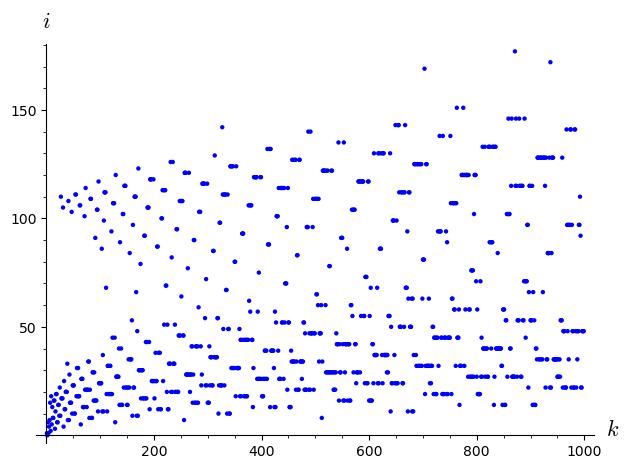
\includegraphics[scale=0.7]{imgs/collatz.png}
  \caption{Tempo de parada $f^i(k) = 1$}
  \label{img:collatz}
\end{figure}
  

Mesmo que você tenha feito tudo certo, não há garantia que
a sua função \ils{collatz} vai eventualmente chegar em um
resultado $i$. Se a conjectura de Collatz for falsa e existir
um contra exemplo, isto é, algum $k_0 \in \NN$ tal que
$f^i(k_0) \neq 1$ para todo $i \in \NN$, então a sua função
será executada por toda a eternidade. Então se você tentou calcular
\ils{collatz(k)} e o seu programa não retornou resultado
alguma das seguintes opções é verdadeira: 1) você cometeu
algum erro no código (esperamos que não), 2) o seu $k$ é
muito grande e o seu computador ainda está no caminho
(o mais provável), ou 3) parabéns, você encontrou um contra
exemplo para a conjectura de Collatz.

Mesmo que a conjectura de Collatz já tenha sido verificada para
números muito muito grandes, não há garantia que ela seja válida.
Um exemplo clássico disso é uma conjectura de Polya, feita
em 1919, sobre
a paridade da quantidade de divisores até certo número. Embora
a afirmação pareça ser válida ao análisar os
primeiros naturais, um contra exemplo foi encontrado na década
de 60. Hoje sabemos que o menor contra exemplo 
para conjectura de Polya é o número $906\,150\,257$.
Assim, ainda que programas de computador forneçam indícios de
que uma afirmação seja verdade, uma demonstração
é essencial para realmente confirmar sua validade.
Por outro lado, se suspeitarmos que uma afirmação é falsa, 
um contra exemplo encontrado computacionalmente
já garante que afirmação não é verdadeira.


\begin{exercise}
  Pesquise sobre a conjectura de Polya e verifique que ela é
  válida para os primeiros $1000$ naturais.
\end{exercise}

\subsection{Primos Gêmeos}
Vejamos uma lista com os 100 primeiros primos
\begin{sageinput}
print(primes_first_n(100))                                                                         
\end{sageinput}
\begin{sageoutput}
[2, 3, 5, 7, 11, 13, 17, 19, 23, 29, 31, 37, 41, 43, 47, 53, 59, 61, 67, 71, 73, 79, 83, 89, 97, 101, 103, 107, 109, 113, 127, 131, 137, 139, 149, 151, 157, 163, 167, 173, 179, 181, 191, 193, 197, 199, 211, 223, 227, 229, 233, 239, 241, 251, 257, 263, 269, 271, 277, 281, 283, 293, 307, 311, 313, 317, 331, 337, 347, 349, 353, 359, 367, 373, 379, 383, 389, 397, 401, 409, 419, 421, 431, 433, 439, 443, 449, 457, 461, 463, 467, 479, 487, 491, 499, 503, 509, 521, 523, 541]
\end{sageoutput}
Analisando atentamente notamos que os primos parecem se distanciar
uns dos outros a medida que crescem, mas, vez ou outra, existem pares de primos
muito próximos, por exemplo: $107$ e $109$, $239$ e $241$, $419$ e $421$, etc. 
Primos $p<q$ são ditos \emph{gêmeos} se $q = p+2$.
\index{Número!primo!gêmeo}
Faça
os exercícios a seguir e crie sua própria conjectura sobre primos gêmeos.
\index{Conjectura!primos gêmeos}

\begin{exercise}
  Crie um código que conte quantos pares de primos gêmeos existem
  até $1000$. E áté $10\,000$? E $100\,000$?
\end{exercise}

Discutiremos mais sobre primos especiais
e a distribuição dos números primos no Capítulo \ref{chap:primos}.

\subsection{Sequências Recorrentes e Expressões Simbólicas}
\label{par:fib}
A sequência de Fibonacci $(u_n)$ é definida da seguinte forma:
\index{Fibonacci}\index{Sequência!de Fibonacci}
$u_0 = u_1 = 1$ e $u_{n} = u_{n-1} + u_{n-2}$ para $n\geq 2$.
Usando a recursividade podemos calcular o valor de $u_n$ de
forma simples
\begin{sageinput}
def fib(n):
  if n == 0 or n == 1:
    return 1
  return fib(n-1) + fib(n-2)
[fib(n) for n in [0..10]]
\end{sageinput}
\begin{sageoutput}
[1, 1, 2, 3, 5, 8, 13, 21, 34, 55, 89]
\end{sageoutput}
De forma mais geral, uma sequência recorrente linear
de ordem $k$ é uma sequência $(x_n)$ tais que existem
constantes $c_1,\cdots,c_k$ tais que
$$
  x_{n+k} = \sum_{j = 1}^k c_j x_{n+k-j}
$$
para $n \in \NN$. Tais sequências dependem dos seus $k$
primeiros termos.

\begin{exercise} 
  Crie um código sage que calcule o valor de uma
  sequência recorrente linear, como a $(x_n)$ acima,
  dados os seus $k$ primeiros
  termos e as constantes $c_j$, $1\leq j \leq k$.
\end{exercise}

Apesar de apresentarmos a sequência de Fibonacci
de forma recursiva, existe uma forma geral para 
os termos $u_n$:
$$
u_n = \frac{\varphi^n - \psi^n}{\varphi - \psi},\quad
\text{ onde }
\varphi = \frac{1+\sqrt{5}}{2}
\text{ e }
\psi = \frac{1-\sqrt{5}}{2}
$$
A existência de uma fórmula desse tipo vale
para sequências recorrentes lineares mais
gerais, recomendamos a leitura de \cite[Apêndice B]{tnumgugu},
especialmente a Seção B.4 (no caso da fórmula
acima para sequência de Fibonacci, você pode
demonstrar a fórmula por indução).
 O código a seguir
calcula o n-ésimo elemento na sequência de Fibonacci
usando essa fórmula geral.
\begin{sageinput}
def fib_g(n):
    phi = (1+sqrt(5))/2
    psi = (1-sqrt(5))/2
    return (phi^n - psi^n)/(phi-psi)  
print(fib_g(5))
\end{sageinput}
O resultado deveria ser \ils{8}, certo? Mas...

\begin{sageoutput}
1/320*sqrt(5)*((sqrt(5) + 1)^6 - (sqrt(5) - 1)^6)
\end{sageoutput}
Se você estiver usando o \sage em algum notebook
(no cocalc, SageMathCell ou  jupyter), pode pedir
para o \sage mostrar o resultado usando a função
\ils{show} ao inves do \ils{print}
\footnote{No interpretador \sage essa
função irá retornar o código \LaTeX\ da
visualização exibida.}, será exibida a expressão

$$
\newcommand{\Bold}[1]{\mathbf{#1}}\frac{1}{320} \, \sqrt{5}
  {\left({\left(\sqrt{5} + 1\right)}^{6} - {\left(\sqrt{5} - 1\right)}^{6}\right)}
$$
O leitor mais corajoso pode verificar que essa expressão
realmente é igual a $8$. No \sage, podemos obter
esse resultando usando a função \ils{expand}:
\begin{sageinput}
expand(fib_g(6))
\end{sageinput}
\begin{sageoutput}
8
\end{sageoutput}
O resultado \emph{inesperado} é na verdade uma das
vantagens do \sage. Em uma linguagem de programação usual,
como no próprio Python, ao definir 
$\varphi = \frac{1+\sqrt{5}}{2}$, o valor seria convertido
em um número real --- na verdade, no ponto flutuante
que aproxima $\varphi$, induzindo um erro de aproximação ---
depois disso as contas são feitas com essas aproximações.
\textbf{O código abaixo está em linguagem Python, e não
\sage} (por isso foi necessário importar a função \ils{sqrt},
no \sage isso não é necessário).
\begin{sageinput}
>>> from math import sqrt
>>> phi = (1+sqrt(5))/2
>>> print(phi)
>>> print(type(phi))
\end{sageinput}
\begin{sageoutput}
1.618033988749895
<class 'float'>
\end{sageoutput}
% Após isso, as contas são feitas usando esse tipo de dado.
No \sage, por outro lado, o cálculo é feito internamente de
forma simbólica.
Vejamos o tipo de dado que é $\varphi$.
\begin{sageinput}
phi = (1+sqrt(5))/2
parent(phi)                                                                                        
\end{sageinput}
\begin{sageoutput}
Symbolic Ring
\end{sageoutput}
Isso significa que, da forma como foi definido,
\ils{phi} é uma \emph{expressão simbólica}. Você
pode visualizar o valor real (aproximado) de 
$\varphi$ com  \ils{RR(phi)}, mas
há muitas vantagens em se usar expressões simbólicas,
mesmo quando estamos trabalhando apenas com números.
Não usaremos a computação simbólica de forma mais
aprofundada nesse texto, mas a ideia é que os
cálculos são feitos de forma mais parecida com o que nós
(humanos) fazemos (afinal, ao fazer uma conta com 
o $\varphi$ você substituiria seu valor por
$\approx 1.61803398874989...$ e usaria esse número?).
Os exercícios a seguir o guiarão por algumas das
possibilidades do cálculo simbólico
\footnote{Algumas das manipulações
que faremos com expressões simbólicas, quando lidam com expressões
polinomiais, são feitas de forma mais eficiente no
\sage usando outro tipo de objeto, elementos
de anéis de polinômios.}.

\begin{exercise}
  Não apenas números podem ser tratados simbolicamente
  pelo \sage mas, principalmente, variáveis. Por padrão
  a única variável (no sentido computacional) que o \sage
  assume ser uma variável (no sentido matemático) é o
  \ils{x}, mas você pode definir outras variáveis.
  \begin{itemize}
    \item[a)] Crie uma variável $y$ com a função \ils{var('y')} \index[sage]{\ils{var}}
    e verifique o seu tipo usando a função \ils{parent}, como
    fizemos acima.
    \item[b)] Defina $f = x^3 - y^3$ e use a função \ils{factor}
    para encontrar a fatoração de $f$ (sim, é o mesmo \ils{factor}
    que fatora um número em primos!)
    \item[c)] É possível substituir valores em uma
    expressão simbólica. Tente \ils{f.subs(x==2,y==1)}. 
    \item[d)] \ils{derivative(f,y)} deve ser autoexplicativo.
    \index[sage]{\ils{derivative}}
    \index[sage]{\ils{.subs}}
    Mude a expressão para $f$ e calcule sua derivada. Usando
    o método \ils{.subs()} é possível calcular a derivada
    em um ponto específico. O que ocorre
    se tentarmos calcular a derivada em um ponto onde a função
    não é diferenciável? (Dica: no sage $|x|$ pode ser escrito
    como \ils{abs(x)})
    \item[d] Desafio: Construa um código que calcule
    (simbolicamente) a derivada
    de uma função
    sem usar a função \ils{derivative}. (Dica: Crie uma
    nova variável \ils{h}, se lembre da definição de
    derivada e use a função \ils{limit}). \index[sage]{\ils{limit}}
  \end{itemize}
\end{exercise}

\begin{exercise} 
  A função \ils{bool()} verifica se o argumento
  passado é verdadeiro ou falso.
  Tente explicar o que está acontecendo no código a seguir:
  \begin{sageinput}
print(bool(sqrt(x^2) == x))
assume(x>0)
print(bool(sqrt(x^2) == x))
  \end{sageinput}
  \begin{sageoutput}
False
True
  \end{sageoutput}
\end{exercise}

\begin{exercise} 
  Uma das mais importantes aplicações do cálculo
  simbólico é a resolução de equações. 
  \begin{itemize}
    \item[a)] Interprete os resultados de
    \ils{solve(x\^{}5-1,x)}  e \ils{solve(x\^{}7+x\^{}2-2*x+2,x)}.
  \end{itemize}
  \index[sage]{\ils{solve}}
  Vamos
  encontrar a interseção entre o círculo unitário
  $x^2 + y^2 = 1$ e a reta $x+2y = 1$.
  \begin{sageinput}
eqs = [x^2 + y^2 == 1, x+2*y == 1]
solve(eqs,x,y)
  \end{sageinput}
  \begin{sageoutput}
[[x == 1, y == 0], [x == (-3/5), y == (4/5)]]
  \end{sageoutput}
  \begin{itemize}
    \item[b)] Encontre os pontos na interseção entre
    as curvas $y^2 = x^3 + x$ e $y = 3x$.
    \item[c)] Você pode verificar se o resultado
    está correto o substituindo nas equações...
    \item[d)] ... ou pode \emph{verificar} visualmente
    exibindo as curvas e os pontos envolvidos. Por exemplo,
    o ponto $(0,0)$ é um ponto na interseção.
    \begin{sageinput}
var('y')
c1 = implicit_plot(y^2 == x^3 + x,(-1,1),(-1,1),color='green') 
c2 = implicit_plot(y == 3*x,(-1,1),(-1,1),color='red')
p = point((0,0),size=40,color='black')
show(c1+c2+p)
    \end{sageinput}
    \begin{figure}[h]
      \centering
      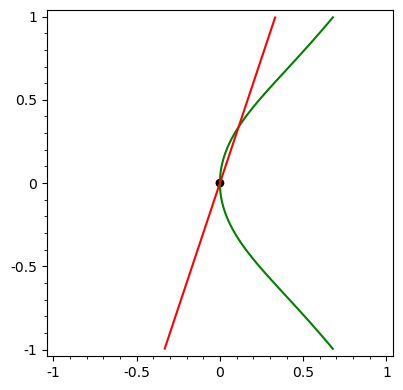
\includegraphics[scale=0.6]{imgs/cepoints.png}
      \caption{Interseção entre $y^2 = x^3 + x$ e $y = 3x$}
      \label{img:cepoints}
    \end{figure}
  \end{itemize}
    O resultado está na Figura \ref{img:cepoints}. Os
    \ils{(-1,1)} representam os intervalos de $x$ e $y$ no gráfico.
    Assim o código \ils{implicit\_plot(eq,(a,b),(c,d))} vai
    \index[sage]{\ils{implicit\_plot}}
    exibir o gráfico da equação implícita nas variáveis $x$ e $y$
    dada em \ils{eq} no retângulo $[a,b]\times[c,d]$, isto é,
    $a\leq x \leq b$ e $c\leq y \leq d$.
    Para uma das soluções do item $d)$ você vai precisar
    alterar o intervalo para conseguir visualizar o ponto.
    \index{Gráfico!Curva implícita}
\end{exercise}

\begin{exercise} 
  Use a técnica apresentada em \cite[B.4]{tnumgugu} para 
  encontrar a fórmula geral da recorrência
  $x_n = 4x_{n-1} + 3x_{n-2} - 14x_{n-3} -6x_{n-4}$ com termos
  iniciais $x_0 = x_1 = 4, x_2 = 22$ e $x_3 = 58$.
\end{exercise}


Apesar de não entrarmos em muitos detalhes, o
cálculo simbólico é uma das ferramentas mais úteis do \sage. 
\index{Cálculo Simbólico}
A documentação oficial possui uma extensa lista de
aplicações, que incluem resolução de equações, cálculos
envolvendo derivadas,
integrais, séries, etc. Veja \cite[Symbolic Calculus]{sagedoc}.




\section{Exercícios}
\begin{exercise} 
  Crie um código \sage que funcione como a função
  \ils{divisors}. Tente otimizar o seu código
  (Veja o item \textit{b)} do Exercício \ref{ex:fatoracaoprimos}).
\end{exercise}

\begin{exercise} 
  \label{ex:fatorial}
  Use a recursividade para criar uma função que calcule o fatorial de
  um número. Siga as instruções:
  \begin{itemize}
    \item[a)] Defina uma função meu\_fatorial com a
    com assinatura \ils{def meu\_fatorial(n):}
    \item[b)] Teste se $n = 0$, nesse caso a função
    deve retornar o valor $1$.
    \item[c)] Se $n>1$, a função deve retornar
    $n\times(n-1)!$, isto é,  \ils{n*meu\_fatorial(n-1)}.
  \end{itemize}
\end{exercise}

\begin{exercise} 
  Use a recursividade para calcular o $\mdc$ entre dois inteiros
  não ambos nulos. Use o Lema \ref{lemma:mdc}.
\end{exercise}

\begin{exercise}
  \label{ex:fatoracaoprimos}
  Reescreva um algoritmo que encontre a fatoração
  de um natural $n>1$ com as otimizações discutidas. Atente
  para os itens a seguir.
  \begin{itemize}
    \item[a)] Remova o uso da recursividade, dessa forma você
    pode criar uma lista \ils{fatores} dentro da própria função
    e armazenar os fatores primos encontrados.
    \item[b)] Prove que se $p$ é o menor primo dividindo
    $n$, então $p \leq \sqrt{n}$. Use esse fato para limitar superiormente
    a busca pelos fatores primos de n.
    \item[c)] Prove que se $p$ é o menor primo dividindo $n$,
    então nenhum primo menor que $p$ divide $n/p$.  Use esse
    fato para limitar inferiormente a busca pelos fatores primos de n.
  \end{itemize}
\end{exercise}

\begin{exercise}
  XGCD de forma mais direta 
\end{exercise}

\begin{exercise}
  O algoritmo de Euclides estendido pode ser descrito na forma
  matricial. Iniciamos com a matriz
  $$M = \begin{pmatrix}
    x_0 & x_1 \\
    y_0 & y_1 \\
    r_0 & r_1
  \end{pmatrix}
  = \begin{pmatrix}
    1 & 0 \\
    0 & 1 \\
    a & b
  \end{pmatrix}.
  $$
  Agora, enquanto $r_1 \neq 0$, tome $q = \lfloor r_0/r_1\rfloor$,
  e alteramos a matriz $M$ da seguinte forma:
  $$
    M \longleftarrow M 
    \begin{pmatrix}
      0 & 1 \\
      1 & -q
    \end{pmatrix}.
  $$
  Verifique que, ao final do processo teremos que $r_0 = \mdc(a,b)$ e
  $x_0a+y_0b = \mdc(a,b)$. 
  Pesquise sobre a manipulação de matrizes no \sage e implemente
  o algoritmo de Euclides estendido da forma descrita acima. (Note que não
  é preciso definir variáveis auxiliares $x_0,x_1,y_0,\dots$, todas as informações
  estão contidas na matriz $M$ e em $q$.)
\end{exercise}

\begin{exercise}
  Dada uma fração contínua $[a_0;a_1,a_2,a_3,\dots]$, sua
  $n$-ésima convergente $p_n/q_n$ pode ser calculada 
  através da relação de recorrência
  % Crie um código que retorne a $n$-ésima convergente $p_n/q_n$ de uma
  % fração contínua $[a_0;a_1,a_2,a_3,\dots]$ usando as relações
  % de recorrência
  $$
  \begin{cases}
    p_n = a_np_{n-1} + p_{n-2} \\
    q_n = a_nq_{n-1} + q_{n-2} \\
  \end{cases}
  $$
  \begin{itemize}
    \item[a)] As relações acima são conhecidas como fórmulas de Wallis.
    Dê uma demonstração usando indução.
    \item[b)] Crie um código que calcule a $n$-ésima convergente
    usando as fórmulas de Wallis. Compare o resultado do seu código
    com o obtido pelo método \ils{.convergent}.
    (Dica: você pode tratar uma fração contínua  como uma lista para obter seus termos,
  por exemplo, \ils{continued\_fraction(pi)[4]} retorna \ilso{292}.)
  \end{itemize}

  
\end{exercise}


\begin{exercise}
  Um bom aluno de álgebra abstrata deve ter notado que existem
  muitas semelhanças entre o anel dos inteiros $\ZZ$ e o anel dos
  polinômios em uma indeterminada com coeficientes em um corpo, por exemplo, $\QQ[t]$.
  Por exemplo, é possível efetuar a divisão euclidiana
  de um polinômio por outro (não nulo), com condições análogas de unicidade,
  você também pode calcular o $\mdc$ entre polinômios, fatorá-los, etc.
  O \sage consegue manipular polinômios tão bem quanto manipula
  os inteiros. Para trabalhar com os polinômios precisamos primeiramente
  definir o ambiente em que eles estão (já que, como os números, 
  um polinômio com a mesma expressão pode ser considerado
  como elemento de vários aneis distintos), sobre os racionais, por
  exemplo, podemos definir $\QQ[t]$ com
  o comando \ils{P.<t>  = QQ[]}. Ao mesmo tempo que
  estamos definindo \ils{P} $= \QQ[t]$, também estamos indicando
  ao \sage que, a partir de agora, \ils{t} deve ser considerado como
  a indeterminada do anel $\QQ[t]$.
  Na célula a seguir definimos o anel
  $\QQ[t]$, e exploramos o polinômio $f(t) = t^6 - 1 \in \QQ[t]$. Não exibimos
  o resultado.
\begin{sageinput}
P.<t> = QQ[t]
f = P(t^6 - 1)
print(f)
print(f(5))
print(f.quo_rem(P(t^2 - 1)))
print(f.quo_rem(P(t^4+2*t)))
print(f.is_irreducible())
print(factor(f))
f.roots()
f.roots(QQbar)
\end{sageinput}
\begin{itemize}
  \item[a)] Execute as funções acima e interprete o resultado. 
  \item[b)] Pesquise por mais funções disponíveis para polinômios.
  \item[c)] Teste a aritmética para polinômios sobre outros anéis.
 \end{itemize}
\end{exercise}

\begin{exercise}
  Pesquise sobre a função \ils{timeit} ou o comando mágico
  \ils{\%timeit}. COMPARAR OS TEMPOS DE EXECUÇÃO
  \index[sage]{\ils{timeit}}
\end{exercise}
